\documentclass[aspectratio=169,11pt]{beamer}

\usetheme{Boadilla}
\usecolortheme{dolphin}
\usefonttheme{professionalfonts}
\setbeamertemplate{navigation symbols}{}
\setbeamertemplate{footline}[frame number]

\usepackage[T1]{fontenc}
\usepackage{lmodern}
\usepackage{amsmath,amssymb,mathtools}
\usepackage{mathpartir}
\usepackage{booktabs,array}
\usepackage{tikz}
\usetikzlibrary{arrows.meta,positioning,calc}

\definecolor{DeepBlue}{HTML}{1F4E79}
\definecolor{SoftBlue}{HTML}{E9F2FA}
\definecolor{SoftGold}{HTML}{FFF2CC}
\definecolor{SoftGreen}{HTML}{E2F0D9}
\definecolor{SoftRed}{HTML}{FCE4D6}
\definecolor{DarkGray}{HTML}{404040}

\setbeamercolor{title}{fg=DeepBlue}
\setbeamercolor{frametitle}{fg=DeepBlue}
\setbeamercolor{block title}{bg=DeepBlue,fg=white}
\setbeamercolor{block body}{bg=SoftBlue,fg=black}
\setbeamercolor{alerted text}{fg=DeepBlue}

\newcommand{\Proc}{\mathrm{Pr}}
\newcommand{\Rew}{\mathrm{R}}
\newcommand{\Nm}{\mathrm{Nm}}
\newcommand{\rw}{\rightsquigarrow}
\newcommand{\ty}{\mathrel{::}}
\newcommand{\dep}{\mathsf{\Pi}}
\newcommand{\app}{\mathsf{app}}
\newcommand{\lam}{\mathsf{lam}}
\newcommand{\Lam}{\mathsf{lam}^{\sharp}}
\newcommand{\out}{\mathsf{out}}
\newcommand{\inp}{\mathsf{in}}
\newcommand{\Inp}{\mathsf{in}^{\sharp}}
\newcommand{\parop}{\mathsf{par}}
\newcommand{\comm}{\mathsf{comm}}
\newcommand{\Dia}{\Diamond}
\newcommand{\hole}{[-]}
\newcommand{\Sig}{\Sigma}
\newcommand{\Hyp}{\mathsf{Hyp}}
\newcommand{\Mod}[4]{\left\langle #1\right\rangle^{#2}_{#3} #4}

\title[Operational hypercubes]{Deriving Hypercubes of Type Systems}
\author[Stay, Meredith, Wells]{Michael Stay \and L. Gregory Meredith \and Christian Wells}
\date{}

\begin{document}

% 1
\begin{frame}
  \titlepage
\end{frame}

% 2
\begin{frame}{The question}
\large
Barendregt's Lambda Cube starts with untyped lambda calculus and varies how terms and types may depend on one another.

\vspace{0.8em}
\begin{block}{Question}
Can other operational calculi generate analogous families of type systems?
\end{block}

\vspace{0.4em}
Example target: asynchronous communication in the \(\pi\)-calculus.
\end{frame}

% 3
\begin{frame}{Main thesis}
\begin{center}
\Large The dependent product is generated by an \alert{operational site}.
\end{center}

\vspace{0.8em}
\begin{itemize}
  \item In lambda calculus: the function position of the beta redex.
  \item In other calculi: any declared source occurrence of a redex.
  \item The result: a hypercube of modal dependent typing disciplines.
\end{itemize}
\end{frame}

\begin{frame}{Barendregt's dependent product rules}
\small

Fix a set of allowed product profiles
\[
  \mathcal S \subseteq \{\ast,\square\}\times\{\ast,\square\}.
\]
Each pair \((s_1,s_2)\in\mathcal S\) licenses a dependent product whose
domain has sort \(s_1\) and whose codomain has sort \(s_2\).

\vspace{1em}

\begin{columns}[T,onlytextwidth]
\begin{column}{0.48\textwidth}
\begin{block}{Formation}
\[
\inferrule*[right={\(\Pi\)-form}]
  {
    \Gamma \vdash A : s_1 \quad
    \Gamma,x:A \vdash B : s_2
  }
  {
    \Gamma \vdash \Pi_{x:A} B : s_2
  }
\]
\end{block}
\end{column}

\begin{column}{0.48\textwidth}
\begin{block}{Introduction}
\[
\inferrule*[right={\(\Pi\)-intro}]
  {
    \Gamma \vdash A : s_1 \quad
    \Gamma,x:A \vdash B : s_2 \\
    \Gamma,x:A \vdash C : B
  }
  {
    \Gamma \vdash \lambda x:A.C : \Pi_{x:A} B
  }
\]
\end{block}
\end{column}
\end{columns}

\vspace{1em}

\begin{center}
\footnotesize
Different choices of \(\mathcal S\) give the systems of the Lambda Cube.
\end{center}

\end{frame}

% 5
\begin{frame}{The cube}
    \begin{center}
    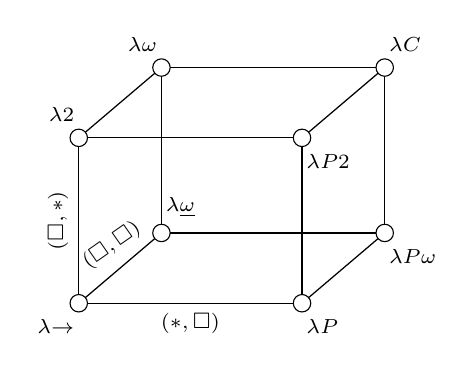
\begin{tikzpicture}[
      scale=1.05,
      every node/.style={transform shape},
      cubept/.style={
        circle,
        draw,
        fill=white,
        inner sep=1.5pt,
        minimum size=6pt
      },
      calc/.style={
        font=\scriptsize,
        align=center
      },
      edge/.style={line width=0.45pt}
    ]

    % Coordinates: base square plus shifted top square.
    % Dimensions correspond informally to adding the three non-base profiles:
    % (*,\square), (\square,*), and (\square,\square).
    \coordinate (A) at (0,0);       % lambda->
    \coordinate (B) at (2.7,0);     % lambda-2
    \coordinate (C) at (0,2.0);     % lambda-omega
    \coordinate (D) at (2.7,2.0);   % lambda-P
    \coordinate (E) at (1.0,0.85);  % lambda-underline-omega
    \coordinate (F) at (3.7,0.85);  % lambda-C
    \coordinate (G) at (1.0,2.85);  % lambda-P2
    \coordinate (H) at (3.7,2.85);  % lambda-C2

    % Edges
    \draw[edge] (A) -- (B) -- (D) -- (C) -- (A);
    \draw[edge] (E) -- (F) -- (H) -- (G) -- (E);
    \draw[edge] (A) -- (E);
    \draw[edge] (B) -- (F);
    \draw[edge] (C) -- (G);
    \draw[edge] (D) -- (H);

    % Points
    \node[cubept] at (A) {};
    \node[cubept] at (B) {};
    \node[cubept] at (C) {};
    \node[cubept] at (D) {};
    \node[cubept] at (E) {};
    \node[cubept] at (F) {};
    \node[cubept] at (G) {};
    \node[cubept] at (H) {};

    % Labels
    \node[calc, below left=2pt and -2pt of A] {\(\lambda{\to}\)};
    \node[calc, below right=2pt and -2pt of B] {\(\lambda P\)};
    \node[calc, above left=2pt and -2pt of C] {\(\lambda 2\)};
    \node[calc, below right=2pt and -2pt of D] {\(\lambda P2\)};

    \node[calc, above right=2pt and -2pt of E] {\(\lambda\underline{\omega}\)};
    \node[calc, below right=2pt and -2pt of F] {\(\lambda P\omega\)};
    \node[calc, above left=2pt and -2pt of G] {\(\lambda \omega\)};
    \node[calc, above right=2pt and -2pt of H] {\(\lambda C\)};

    % Optional axis/profile labels
    \node[calc] at (1.35,-0.25) {\((\ast,\square)\)};
    \node[calc, rotate=90] at (-0.25,1.0) {\((\square,\ast)\)};
    \node[calc, rotate=35] at (0.4,0.7) {\((\square,\square)\)};

    \end{tikzpicture}
    \end{center}

\begin{center}
\begin{tabular}{c c c}
\toprule
Profile & Reading & Dependency\\
\midrule
\((\ast,\ast)\) & ordinary functions & terms on terms \\
\((\ast,\square)\) & dependent types & types on terms \\
\((\square,\ast)\) & polymorphism & terms on types \\
\((\square,\square)\) & type operators & types on types \\
\bottomrule
\end{tabular}
\end{center}
\end{frame}

% 6
\begin{frame}{Where does \(\Pi\) come from?}
\begin{center}
\Large A function is useful because application exposes a computation.
\end{center}

\vspace{0.5em}
\[
  \app(\lam(t),a)\rw t(a)
\]

\vspace{0.5em}
\begin{columns}[T]
\begin{column}{0.48\textwidth}
\begin{block}{Selected source subterm}
\[
  U=\lam(t)
\]
\end{block}

\end{column}
\begin{column}{0.48\textwidth}
\begin{block}{Surrounding context}
\[
  K\hole=\app(\hole,a)
\]
\end{block}
\end{column}
\end{columns}
\end{frame}

% 7
\begin{frame}{Why modal?}
Ordinary product elimination suggests type preservation.

\[
  f: \Pi_{x:A}B,\quad a:A
  \quad\leadsto\quad
  f\,a:B[a/x]
\]

\vspace{0.8em}
For general operational theories, we usually only get a \alert{one-step may property}:


\begin{block}{Modal reading}
\[
  P \rw Q
  \quad\text{and}\quad
  Q\ty C
  \quad\text{imply}\quad
  P\ty\Dia C
\]
\end{block}
$P$ may step to something of type $C.$
\end{frame}

% 8
\begin{frame}{Input: finite operational presentations}

\vspace{0.5em}
\begin{columns}[T]
\begin{column}{0.48\textwidth}
\begin{block}{Presentation data}
\begin{itemize}
  \item carriers: \(\Proc,\Rew,\ldots\)
  \item term constructors
  \item structural equations
  \item primitive rewrite constructors
\end{itemize}
\end{block}

\end{column}
\begin{column}{0.48\textwidth}
\begin{block}{Extra design data}
\begin{itemize}
  \item displayed source sites
  \item profile-matching constraints
  \item allowed local profiles
  \item closure support, when needed
\end{itemize}
\end{block}
\end{column}
\end{columns}
\end{frame}

% 9
\begin{frame}{Example operational theory: lambda calculus}
\begin{block}{Wrapped syntax}
\[
  \app:\Proc\times\Proc\to\Proc,
  \qquad
  \lam:\Proc^{\Proc}\to\Proc
\]
\end{block}

\begin{block}{Primitive beta step}
\[
  p:\Proc,\; k:\Proc\to\Proc
  \vdash
  \app(\lam(k),p)\rw k(p)
\]
\end{block}

\begin{block}{Chosen evaluation support}
A head-context closure rule propagates rewrites through function position.
\end{block}
\end{frame}

% 10
\begin{frame}{Example operational theory: asynchronous \(\pi\)}
\begin{block}{Core syntax}
\[
\begin{array}{rcl}
  \mathrm{nil} &:& \Proc \\
  p\mid q &:& \Proc \\
  n!m &:& \Proc \\
  n?k &:& \Proc \\
  !p,\; \nu k &:& \Proc
\end{array}
\]
\end{block}

\begin{block}{Communication}
\[
  n!m\mid n?k \rw k(m)
\]
\end{block}
\end{frame}

% 11
\begin{frame}{Concurrency changes the typing problem}
\begin{center}
\Large A process may have many possible futures.
\end{center}

\vspace{0.6em}
\begin{itemize}
  \item Parallel composition is commutative and associative.
  \item A race has inequivalent outcomes.
  \item Useful properties are often about \alert{what may happen next}.
\end{itemize}

\vspace{0.6em}
\[
  \text{receive type} \;\neq\; \text{invariant type}
\]
\end{frame}

% 12
\begin{frame}{Declared sites}
\begin{center}
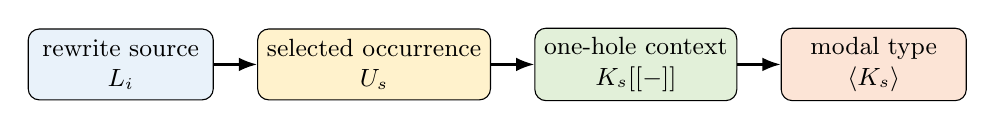
\begin{tikzpicture}[node distance=0.55cm, every node/.style={align=center, font=\small}, >=Latex]
  \node[draw,rounded corners,fill=SoftBlue,minimum width=2.35cm,minimum height=0.9cm] (source) {rewrite source\\\(L_i\)};
  \node[draw,rounded corners,fill=SoftGold,minimum width=2.35cm,minimum height=0.9cm,right=of source] (site) {selected occurrence\\\(U_s\)};
  \node[draw,rounded corners,fill=SoftGreen,minimum width=2.35cm,minimum height=0.9cm,right=of site] (context) {one-hole context\\\(K_s[\hole]\)};
  \node[draw,rounded corners,fill=SoftRed,minimum width=2.35cm,minimum height=0.9cm,right=of context] (type) {modal type\\\(\langle K_s\rangle\)};
  \draw[->,thick] (source) -- (site);
  \draw[->,thick] (site) -- (context);
  \draw[->,thick] (context) -- (type);
\end{tikzpicture}
\end{center}

\vspace{0.6em}
\begin{block}{Key design choice}
Sites are selected displayed occurrences, not all subterms modulo equations.
\end{block}
\end{frame}

% 13
\begin{frame}{Three classes of site variables}
For a site \(s\), factor the source as \(L_i=K_s[U_s]\).

\vspace{0.5em}
\begin{columns}[T]
\begin{column}{0.32\textwidth}
\begin{block}{Index}
Shared by \(U_s\) and \(K_s\).
\[
  \vec x_s=\mathrm{FV}(U_s)\cap\mathrm{FV}(K_s)
\]
\end{block}

\end{column}
\begin{column}{0.32\textwidth}
\begin{block}{Rely}
Supplied by the context only.
\[
  \vec y_s=\mathrm{FV}(K_s)\setminus\mathrm{FV}(U_s)
\]
\end{block}

\end{column}
\begin{column}{0.32\textwidth}
\begin{block}{Ambient}
Parameters of the selected term or target.
\[
  \vec z_s\text{ stays outside}
\]
\end{block}
\end{column}
\end{columns}
\end{frame}

% 14
\begin{frame}{Comparison I: redex, site, context}
\small
\begin{tabular}{>{\bfseries}p{0.24\textwidth}p{0.33\textwidth}p{0.33\textwidth}}
\toprule
 & Lambda completion & \(\pi\)-calculus receive completion \\
\midrule
Operational redex
& \(\app(\lam(t),a)\rw t(a)\)
& \(n!m\mid n?k\rw k(m)\) \\
\addlinespace
Declared source site
& function position \(\lam(t)\)
& input occurrence \(n?k\) \\
\addlinespace
Displayed context
& \(K\hole=\app(\hole,a)\)
& \(K\hole=n!m\mid\hole\) \\
\bottomrule
\end{tabular}
\end{frame}

% 15
\begin{frame}{Comparison II: site variables}
\small
\begin{tabular}{>{\bfseries}p{0.24\textwidth}p{0.33\textwidth}p{0.33\textwidth}}
\toprule
 & Lambda completion & \(\pi\)-calculus receive completion \\
\midrule
Index variables
& none for the product site
& channel name \(n\) \\
\addlinespace
Rely variables
& argument \(a\)
& communicated name \(m\) \\
\addlinespace
Ambient variables
& abstraction body \(t:\Proc\to\Proc\)
& continuation \(k:\Nm\to\Proc\) \\
\bottomrule
\end{tabular}

\vspace{0.8em}
\begin{block}{Reading}
Index data remain fixed outside the modality; rely data are supplied when the context is supplied.
\end{block}
\end{frame}

% 16
\begin{frame}{Comparison III: generated contextual type}
\begin{columns}[T]
\begin{column}{0.48\textwidth}
\begin{block}{Lambda}
\[
  \Pi_{x:A}B
\]
\vspace{-0.7em}
\[
  \text{is shorthand for}
\]
\[
  \Mod{\app(\hole,x)}{}{x\ty A}{B}
\]
\end{block}

\end{column}
\begin{column}{0.48\textwidth}
\begin{block}{Receive}
\[
  \Mod{n!m\mid\hole}{n\ty A}{m\ty B}{C}
\]
\vspace{0.3em}
An input process that can communicate with a matching output and reach \(C\).
\end{block}
\end{column}
\end{columns}
\end{frame}

% 17
\begin{frame}{Comparison IV: introduction principles}
\small
\begin{columns}[T]
\begin{column}{0.48\textwidth}
\begin{block}{Lambda abstraction}
If the body has type \(B\) under \(x\ty A\), then:
\[
\begin{array}{c}
  x\ty A \vdash t(x)\ty B\\[2pt]
  \hline
  \Lam(A,t)\ty \Pi_{x:A}B
\end{array}
\]
\end{block}

\end{column}
\begin{column}{0.48\textwidth}
\begin{block}{Input}
Let \(M=\Mod{n!m\mid\hole}{n\ty A}{m\ty B}{C}\). If the continuation has type \(C\), then:
\[
\begin{array}{c}
  n\ty A,\;m\ty B \vdash k(m)\ty C\\[2pt]
  \hline
  n?_B k\ty M
\end{array}
\]
\end{block}
\end{column}
\end{columns}
\end{frame}

% 18
\begin{frame}{Comparison V: elimination is effectful}
\small
\begin{columns}[T]
\begin{column}{0.48\textwidth}
\begin{block}{Application}
\[
\begin{array}{c}
  f\ty \Pi_{x:A}B \qquad a\ty A\\[2pt]
  \hline
  \app(f,a)\ty\Dia(B[a/x])
\end{array}
\]
\end{block}

\end{column}
\begin{column}{0.48\textwidth}
\begin{block}{Communication}
Let \(M=\Mod{n!m\mid\hole}{n\ty A}{m\ty B}{C}\).
\[
\begin{array}{c}
  P\ty M \qquad a\ty B\\[2pt]
  \hline
  n!a\mid P\ty\Dia(C[a/m])
\end{array}
\]
\end{block}
\end{column}
\end{columns}

\end{frame}

% 19
\begin{frame}{Comparison VI: local hypercubes}
\begin{columns}[T]
\begin{column}{0.48\textwidth}
\begin{block}{Product site}
Two profile slots:
\[
  (u,v)\in\{\ast,\square\}^2
\]
Based choices give $2^{2^2 - 1} = 2^3$ calculi.
\end{block}

\end{column}
\begin{column}{0.48\textwidth}
\begin{block}{Receive site}
Three carrier-sensitive slots:
\[
  (\alpha,\beta;\gamma)
  \in
  \{\ast,\square\}_{n}
  \times
  \{\ast,\square\}_{m}
  \times
  \{\ast,\square\}_{C}
\]
Based choices give \(2^{2^3 - 1} = 2^ 7\) calculi.
\end{block}
\end{column}
\end{columns}
\end{frame}

% 20
\begin{frame}{Profile computation}
\begin{center}
\Large Profiles say which sort levels may appear in a site interface.
\end{center}

\vspace{0.6em}
\begin{itemize}
  \item Raw slots: index variables, rely variables, and target type.
  \item Matching data may identify slots.
  \item Quotient profiles are raw profiles constant on identified slots.
  \item A signature choice selects which quotient profiles are allowed.
\end{itemize}

\vspace{0.5em}
\begin{block}{Important separation}
Structural equations transport rewrites; they do not silently move holes or identify profile slots.
\end{block}
\end{frame}

% 21
\begin{frame}{Algorithm skeleton}
\begin{enumerate}
  \item Start with a finite operational presentation.
  \item Choose displayed source sites.
  \item Factor each selected source as \(L_i=K_s[U_s]\).
  \item Compute index, rely, and ambient telescopes.
  \item Compute quotient profile spaces and choose signatures.
  \item Freely add modal type formers and rules.
\end{enumerate}

\vspace{0.5em}
\begin{center}
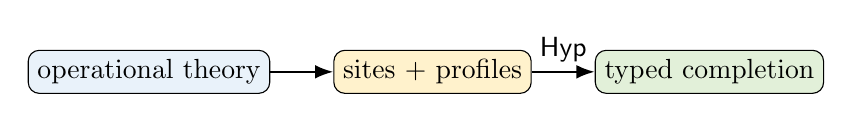
\begin{tikzpicture}[node distance=0.8cm, >=Latex]
  \node[draw,rounded corners,fill=SoftBlue] (op) {operational theory};
  \node[draw,rounded corners,fill=SoftGold,right=of op] (sites) {sites + profiles};
  \node[draw,rounded corners,fill=SoftGreen,right=of sites] (typed) {typed completion};
  \draw[->,thick] (op) -- (sites);
  \draw[->,thick] (sites) -- node[above]{\(\Hyp\)} (typed);
\end{tikzpicture}
\end{center}
\end{frame}

% 22
\begin{frame}{What the completion adds}
\begin{columns}[T]
\begin{column}{0.48\textwidth}
\begin{block}{New syntax}
\begin{itemize}
  \item sort constants \(\ast^X,\square^X\)
  \item typing evidence \(P\ty A\)
  \item possibility \(\Dia C\)
  \item contextual modalities \(\langle K_s\rangle\)
\end{itemize}
\end{block}

\end{column}
\begin{column}{0.48\textwidth}
\begin{block}{New rules}
\begin{itemize}
  \item formation and introduction
  \item modal elimination
  \item source-subterm introduction
  \item computation rules for canonical sources
\end{itemize}
\end{block}
\end{column}
\end{columns}

\vspace{0.5em}
One contextual type former per site; profiles select allowed rule instances.
\end{frame}

% 23
\begin{frame}{Lambda completion: nearly the Lambda cube}
\begin{block}{Product-site completion}
\[
  \dep(A,\lambda x.B) := \Mod{\app(\hole,x)}{}{x\ty A}{B}
\]
\end{block}

\begin{itemize}
  \item The constructor fragment recovers the product-profile geometry.
  \item Erasing \(\Dia\) maps it to the corresponding Barendregt system.
  \item The full modal theory is finer and more operational.
\end{itemize}

\vspace{0.5em}
\[
  (\Dia^n C)^\circ=C^\circ
  \qquad
  \app(f,a)\ty\Dia(B[a/x])
\]
\end{frame}

% 24
\begin{frame}{Receive completion: a communication type}
\begin{block}{Receive-site completion}
\[
  n?_B k
  \ty
  \Mod{n!m\mid\hole}{n\ty A}{m\ty B}{C}
\]
\end{block}

\begin{itemize}
  \item The channel \(n\) is indexed.
  \item The message \(m\) is supplied by the context.
  \item The continuation \(k\) remains ambient.
\end{itemize}

\vspace{0.5em}
\begin{center}
When paired with a matching output, the input may take one communication step to \(C\).
\end{center}
\end{frame}

% 25
\begin{frame}{May-properties, not must-properties}
\begin{columns}[T]
\begin{column}{0.48\textwidth}
\begin{block}{Generated modal typing}
\[
  P\ty\Dia C
\]
means evidence for some:
\[
  P\rw Q
  \qquad
  Q\ty C.
\]
\end{block}

\end{column}
\begin{column}{0.48\textwidth}
\begin{block}{Must property}
\[
  \forall Q.\; P\rw Q\Rightarrow Q\in C
\]
This is model-theoretic and not generated by the local rules alone.
\end{block}
\end{column}
\end{columns}
\end{frame}

% 26
\begin{frame}{Correct by construction}
The main metatheorems are formal consequences of the generated presentation.

\vspace{0.5em}
\begin{block}{Freeness}
The completion adds exactly the chosen generated structure, with no hidden rules.
\end{block}

\begin{block}{Functoriality}
Morphisms of site-and-signature presentations map to morphisms of completions.
\end{block}

\begin{block}{Soundness}
Every derivation has proof-relevant evidence in every structured model.
\end{block}
\end{frame}

% 27
\begin{frame}{Takeaways}
\begin{enumerate}
  \item Dependent products can be read as contextual may-types generated by the beta site.
  \item The same recipe applies to non-lambda operational theories.
  \item The \(\pi\)-calculus receive site yields a communication hypercube.
  \item The algorithm separates displayed syntax, structural equations, and profile choices.
  \item The categorical and semantic theorems certify the construction.
\end{enumerate}
\end{frame}

% 28
\begin{frame}{End}
\begin{center}
\Huge Questions?
\end{center}
\end{frame}

\end{document}
